%% Document created 26 April 2022 automatically 
%% from /Users/massimosotgia/Desktop/uni_at_DIFI/Lab2/setup.py 

%% Copyright (C) Mattia Sotgia et al. 2022
%% Using class revtex4-2.cls
%                                       
%                                       
%██       █████  ██████         ██████  
%██      ██   ██ ██   ██             ██ 
%██      ███████ ██████          █████  
%██      ██   ██ ██   ██        ██      
%███████ ██   ██ ██████  ██     ███████ 
%                                       
%                                       
\documentclass[
    prl,
    % preprint,
    % linenumbers,
    % tightlines,
    reprint, 
    superscriptaddress, 
    altaffilletter, 
    amsmath, 
    amssymb, 
    a4paper,
    varvw]{revtex4-2}

\usepackage[top=1.75cm,bottom=2.5cm,left=1.5cm,right=1.5cm]{geometry}

\usepackage[utf8]{inputenc}
\usepackage[T1]{fontenc}

\usepackage[italian]{babel}

%% revtex4-2 bug-fix
\def\andname{e}
%--------------------
\makeatletter
\let\it@comma@def\active@comma
\makeatother

\usepackage{txfonts}
\usepackage{graphicx}% Include figure files
\graphicspath{{../fig/}}

\usepackage{dcolumn}% Align table columns on decimal point
\usepackage{bm}% bold math
\usepackage[colorlinks, urlcolor=., bookmarks]{hyperref}% add hypertext capabilities
\renewcommand\UrlFont{\color{blue}}

\usepackage{physics}
\usepackage{siunitx}

\usepackage{fancyhdr}
\pagestyle{fancy}
\fancyhf{}
\def\twodigits#1{\ifnum#1<10 0\fi\the#1}

%-----------------------------------------------------------------------------------------------

\usepackage{background}
\SetBgColor{gray}
\SetBgAngle{90}
\SetBgScale{2}
\SetBgVshift{0.27\textwidth}

\usepackage[american resistors]{circuitikz}
\usepackage{listings}
\lstset{
  basicstyle=\fontsize{5}{6}\selectfont\ttfamily,
  % backgroundcolor=\color{white},   % choose the background color
  % basicstyle=\footnotesize,        % the size of the fonts that are used for the code
  breakatwhitespace=false,         % sets if automatic breaks should only happen at whitespace
  breaklines=true,                 % sets automatic line breaking
  captionpos=b,                    % sets the caption-position to bottom
  % commentstyle=\color{mygreen},    % comment style
  deletekeywords={...},            % if you want to delete keywords from the given language
  escapeinside={\%*}{*)},          % if you want to add LaTeX within your code
  % extendedchars=true,              % lets you use non-ASCII characters; for 8-bits encodings only, does not work with UTF-8
  % firstnumber=1000,                % start line enumeration with line 1000
  % frame=single,                    % adds a frame around the code
  % keepspaces=true,                 % keeps spaces in text, useful for keeping indentation of code (possibly needs columns=flexible). 
  % keywordstyle=\color{blue},       % keyword style
  % numbers=left,                    % where to put the line-numbers; possible values are (none, left, right)
  % numbersep=5pt,                   % how far the line-numbers are from the code
  numberstyle=\tiny\color{gray}, % the style that is used for the line-numbers
  % rulecolor=\color{black},         % if not set, the frame-color may be changed on line-breaks within not-black text (e.g. comments (green here))
  showspaces=false,                % show spaces everywhere adding particular underscores; it overrides 'showstringspaces'
  showstringspaces=false,          % underline spaces within strings only
  showtabs=false,                  % show tabs within strings adding particular underscores
  stepnumber=2,                    % the step between two line-numbers. If it's 1, each line will be numbered
  % stringstyle=\color{mymauve},     % string literal style
  tabsize=2,                       % sets default tabsize to 2 spaces
}
\usepackage{soul}


%% Define ref types
\newcommand{\reftab}[1]{Tabella {\ref{#1}}}%
\newcommand{\reffig}[1]{Figura {\ref{#1}}}%
\newcommand{\refeqn}[1]{({\ref{#1}})}%
\newcommand{\ChiSqr}{$\chi^2$\space}
\newcommand{\ChiNdf}{$\chi^2/\text{ndf}$}
\newcommand{\cernroot}{\texttt{root}}
\newcommand{\treSigma}{$3\sigma$}
\newcommand{\stdErr}[1]{$\varepsilon_{#1}$}
\newcommand{\mstdErr}[1]{\varepsilon_{#1}}
%% PAPER ONLY custom Macros

\newenvironment{methods}[1]{\section*{#1}
%\fontfamily{phv}
\fontsize{7.5}{9}\selectfont\label{sec:methods}\noindent}{\par\noindent}

%\usepackage{lcsec}

\usepackage{chemformula}
\usepackage[caption=false]{subfig}
\usepackage[vlined]{algorithm2e}
\sisetup{
    % separate-uncertainty=true,
    % per-mode=symbol,
    round-mode=uncertainty,
    % exponent-mode = scientific
}

\setcounter{secnumdepth}{2}

\fancyfoot[C]{
    \the\year\twodigits\month\twodigits\day/7-\thepage
}
\fancyhead[C]{RELAZIONE DI LABORATORIO \textbf{
    N. 4 % ! <== CAMBIARE (Nessuna rel. -> 00)
    } (\the\year)
}

\begin{document}

\title{Misura della densità di portatori di carica su sonda tramite effetto Hall
}
\thanks{Esperienza n. 7
}

\author{Francesco Polleri}
\email{s5025011@studenti.unige.it}
\author{Mattia Sotgia}
\email{s4942225@studenti.unige.it}
\collaboration{Gruppo A1}
\affiliation{Dipartimento di Fisica, Università degli Studi di Genova, I-16146 Genova, Italia}

% \author{Michele Giorgi}
% \author{Lorenzo Lucentini}
% \collaboration{Gruppo C6}
% \affiliation{Dipartimento di Fisica, Università degli Studi di Genova, I-16146 Genova, Italia}


\date{presa dati
    11--12 maggio 2022, consegnata in data 
    \today
}

\begin{abstract}
    L'effetto Hall si verifica quando delle cariche transitano attraverso una corrente $i$ che è perpendicolare ad un campo magnetico $B$, tali per cui si viene a creare una tensione lungo il terzo asse ortogonale. Questa tensione è direttamente proporzionale a $i$ e $B$, ed inversamente proporzionale alla carica dei portatori e alla loro densità volumica $\eta$.
    Si vuole misurare la densità di portatori di carica di una sonda di bismuto \ch{^{83}Bi} realizzata per deposizione su film. Questa sonda è inserita nel traferro di un circuito magnetico, dove è sottoposta ad un campo $B_t$. La tensione $V_H$ è misurata direttamente sulla sonda, ottenendo quindi una stima della densità volumica di portatori $\eta=\SI{1.310(175)e+25}{\per\cubic\metre}$. Confrontando con precedenti osservazioni sperimentali (\ref{sec:computing_eta_and_conlusion}) troviamo che il risultato è superiore di circa un fattore 10 rispetto ad altri risultati.
\end{abstract}


\maketitle
\thispagestyle{fancy}
% Rimuovere per consegna
\SetBgContents{
    laboratorio2: e7 [non per la consegna] \today % ! Note di versione
}

%%%% CORPO DEL TESTO
%%%% CORPO DEL TESTO

\section{Introduzione}

Il passaggio di corrente attraverso un sottile strato conduttore comporta la presenza di una densità di corrente, attraverso il materiale stesso, $\vec{J}=nq\vec{v}_d$, dove $\vec{v}_d$ è la velocità di drift (o di spostamento) dei portatori di carica, e $\eta$ indica la densità di portatori di carica che contribuiscono alla corrente, per unità di volume, misurata in \si{\per\cubic\metre}. Sottoponendo la lamina conduttrice ad un campo magnetico sufficientemente uniforme \footnote{Il campo magnetico deve essere posto ortogonalmente alla densità di corrente $\vec{J}$, evitando di dover effettuare anche misurazioni dell'angolo $\alpha$ di orientamento di $\vec{B}$ rispetto a $\vec{J}$.} otteniamo che le cariche saranno quindi sottoposte ad una forza di Lorentz \begin{equation}
    \vec{F}_m = q\vec{v}_d \times \vec{B} = qv_dB\hat{u}_H,\label{eq:lorentz_F_m}
\end{equation} che avrà come risultato diretto lo spostamento dei portatori di carica $q$ nella direzione $\hat{u}_H$. Considerando un materiale conduttore come composto da cariche $q$ (portatori di corrente) immersi in una distribuzione che possiamo considerare uniforme (secondo la fisica classica) di cariche $-q$ \footnote{Stiamo considerando il valore di $q$ in termini assoluti, non ponendoci quindi problemi sul segno dei portatori di un conduttore. Un conduttore è però elettricamente neutro, quindi a dei portatori di carica $q$ devono corrispondere delle cariche $-q$ che bilancino complessivamente elettricamente la carica. }, possiamo allora osservare che dopo un certo tempo \footnote{Definiamo questo tempo \emph{tempo caratteristico}, e osserviamo che è sufficientemente piccolo da poter considerare questo processo praticamente istantaneo} si formerà un campo elettrico $\vec{E}_H = \vec{F}_H/q$ in direzione ortogonale a $\vec{J}$ e $\vec{B}$, che comporterà quindi l'esistenza di una differenza di potenziale agli estremi della lamina definita come \begin{equation}
    V_H = \frac{i}{ew}\frac{1}{\eta}B,\label{eq:2}
\end{equation} dove $w$ indica lo spessore della lamina che utilizziamo, che comunque nel nostro apparato sperimentale riusciamo ad avere molto inferiore alle altre dimensioni della sonda utilizzata, e dove $i=JA$ indica il flusso della densità di corrente, ovvero la corrente attraverso una sezione $A$. L'effetto misurato è noto come effetto Hall \cite{Hall_1897}. Misurando la tensione che si viene a creare sulla lamina, possiamo ottenere quindi una misura efficace della densità di portatori in funzione delle altre variabili del nostro setup. 

I portatori di carica di un qualsiasi materiale classico sono elettroni, di carica $e=\SI{1.602176634e-19}{\coulomb}$ \footnote{valore esatto, fonte BIPM, \emph{defining constants}: \url{https://www.bipm.org/en/measurement-units/si-defining-constants}, valore risultato di \cite{Newell_2018}}. 

\section{Metodo sperimentale}
La misura dei portatori di carica viene effettuata utilizzando una sonda di \ch{Bi} metallico costituita da un film sottile depositato su una lamina isolante. Il metodo di deposizione ci permette infatti di avere uno spessore $w$ della lamina piuttosto basso, permettendoci quindi di stabilire in modo univoco quale è la direzione perpendicolare rispetto al piano della sonda, e individuare quindi un sistema destrorso $xyz$ come in figura \ref{fig:sonda.rotated}. Il sistema così individuato può essere utilizzato come riferimento per tutti i calcoli che verranno svolti.

La corrente infatti scorre nel verso negativo di $\hat{e}_1$, che invece è rivolto nella direzione di $\vec{J}$ coerentemente alla direzione della velocità di drift $v_e$ degli elettroni. Tale corrente viene controllata attraverso un generatore calibrato per avere in uscita una corrente costante, ovvero indipendente dal carico, inferiore a \SI{10}{\milli\ampere} per permettere alla sonda di lavorare in condizioni di dissipazione dell'energia verificabili e per avere inoltre fluttuazioni rispetto al valore medio molto inferiori a quelle che si avrebbero collegando semplicemente il generatore da banco, che essendo costruito per un utilizzo generico può non essere la scelta migliore per l'uso specifico di cui necessitiamo. Il generatore di corrente infatti permette di avere un valore di corrente in uscita pari a $\SI{1.7242(300)e-3}{\ampere\per\volt}\times\qty(V_--V_+)$, dove $V_--V_+$ è la differenza di tensione fornita in ingresso al generatore di corrente (per la caratterizzazione del generatore di corrente vedere l'appendice \ref{sec:appendix_current_gen}). Della tensione che forniamo al generatore facciamo una serie di misure insieme alla presa dati e dopo una trattazione di tipo statistico degli errori, troviamo un'incertezza sulla tensione di \SI{2.6}{\milli\volt} e quindi una deviazione standard sulla corrente inferiore a 18 ppt \footnote{Otteniamo una corrente di \SI[separate-uncertainty=true]{8.619(150)}{\milli\ampere}}. 

Lungo $\hat{e}_2$ abbiamo invece il campo magnetico, che sarà realmente la caratteristica chiave dell'apparato. Le caratteristiche di questo campo magnetico sono tali da imporre alcune particolarità nella sua realizzazione. 
%Ciò che adesso ci manca è il campo magnetico a cui sottoponiamo la cariche presenti nella sonda. Per creare tale campo $B$ sono possibili diverse opzioni e noi abbiamo scelto quella di utilizzare un elettromagnete. 
Decidiamo infatti di utilizzare un elettromagnete. Tale strumento ci permette di creare un campo magnetico con un modulo sufficientemente elevato per il tipo di misure che vogliamo effettuare, cosa che una semplice bobina (realizzata con materiali classici) non sarebbe stata in grado di fare. Realizzando un circuito magnetico con traferro possiamo inoltre ottenere una regione di spazio dove ad un primo ordine di approssimazione \footnote{Consideriamo le due superfici sufficientemente grandi e realizzando lo spessore del traferro $\ell_t\ll D_j$, dove con $D_j$ indichiamo una tra le due dimensioni del nucleo ferromagnetico.} possiamo ottenere un campo uniforme al centro e quindi trascurare gli effetti di bordo.  Altra cosa importante è che il campo sia anche facilmente controllabile dalle correnti che scorrono nelle bobine avvolte intorno ai suoi bracci. Se il materiale con cui l'elettromagnete è stato realizzato è ferro dolce allora il suo ciclo di isteresi sarà stretto, per cui possiamo considerare che per valori non troppo elevati di corrente la risposta del campo magnetico sia lineare. Per evitare possibili problemi legati alla magnetizzazione residua decidiamo di effettuare la presa dati fornendo alle bobine dell'elettromagnete valori di corrente sempre decrescenti che, partendo da un valore di \SI{1.2}{\ampere}/\SI{1.3}{\ampere}, scendano sino ad avere corrente nulla \footnote{Nei dati raccolti non abbiamo mai considerato valori della corrente inferiori a \SI{200}{\milli\ampere}} e poi crescano di nuovo in verso opposto \footnote{Quando la corrente arriva al valore minimo, il sistema entra in blocco e attende che manualmente vengano invertiti i cavi che portano la corrente all'elettromagnete}.

\begin{figure}
    \subfloat[][]{\includegraphics[width=0.3\linewidth]{sonda.IMG_0233.png}\label{fig:sonda.IMG}}\hspace{5mm}
    \subfloat[][]{
        \begin{tikzpicture}
            \draw node[inner sep=0] (0) at (-.1,0) {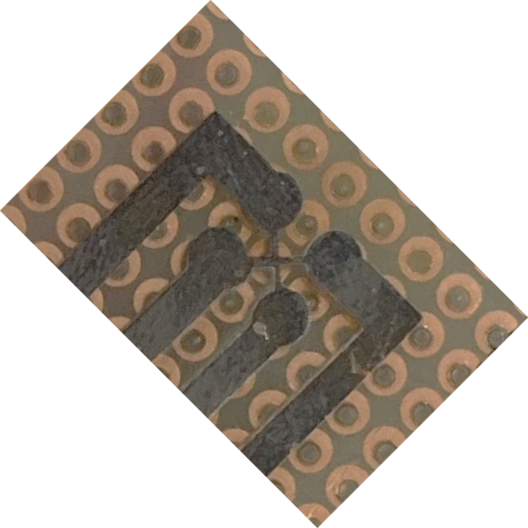
\includegraphics[width=3.5cm]{sonda.IMG_0233_cropped_rotated.png}};
            \draw[-latex, white] (0,.1) to (0,.5) node[above] {$\vu{e}_1$};
            \draw[-latex, white] (.1,0) to (.5,0) node[right] {$\vu{e}_3$};
            \draw[white] (0,0) node[left] {$\vu{e}_2$};
            % \filldraw[white] (0, 0) circle (0.1) 
            \draw node[white] {$\mathbf{\odot}$};
        \end{tikzpicture}
    \label{fig:sonda.rotated}}
    \caption{\ref{sub@fig:sonda.IMG} Dettaglio della sonda utilizzata per misurare l'effetto Hall. In \ref{sub@fig:sonda.rotated} indichiamo anche una terna destrorsa utilizzata per considerazioni fisiche. }\label{fig:misc}
\end{figure}

Dalla legge di Hopkinson \begin{equation}
    \mathcal{F} = \oint \vec{H} \cdot \dd \ell = \Phi \oint \frac{\dd \vec{\ell}}{\mu S} = \Phi \mathcal{R},
\end{equation} definita con \[
    \mathcal{R} = \oint \frac{\dd \vec{\ell}}{\mu S} = \frac{\ell_m}{\mu S}
\] la riluttanza del circuito, possiamo interpretare il circuito magnetico come un circuito elettrico, e quindi, poiché la sezione dell'elettromagnete su tutto l'anello ferromagnetico è sempre la stessa, considerare il traferro come un elemento circuitale con riluttanza $\mathcal{R}_t$ posto in serie. La riluttanza $\mathcal{R}_e$ totale dell'elettromagnete quindi risulterà \begin{equation}
    \mathcal{R}_e = \mathcal{R}_f + \mathcal{R}_t = \frac{\ell_m}{\mu S} + \frac{\ell_t}{\mu_0 S} = \frac{\ell_m + \mu_r\text{(\ch[]{Fe})}\ell_t}{\mu S},
\end{equation} con $\ell_{t}$ lo spessore del traferro e $\ell_{m}$ la lunghezza del circuito magnetico (escluso lo spessore del traferro). Otteniamo quindi il campo magnetico che attraversa la sonda nel traferro \begin{equation}
    B = \frac{iN\mu}{\ell_m + \mu_r\text{(\ch[]{Fe})}\ell_t}.\label{eq:B_i}
\end{equation}

Per ottenere campi magnetici dell'ordine di \SI{0.5}{\tesla}, dall (\ref{eq:B_i}), osserviamo che il valore della corrente che deve essere fornita all'elettromagnete deve essere almeno nell'ordine di \SI{1}{\ampere}. Caratteristica fondamentale di questa corrente è la possibilità di modificarne il valore digitalmente senza dover manualmente cambiarne il valore. Utilizzando quindi una interfaccia seriale di comunicazione possiamo mettere in comunicazione il sistema di controllo del setup sperimentale con il generatore di corrente e quindi controllare in modalità remota il valore della corrente che viene erogata dal generatore \footnote{Per la connessione seriale è necessaria la conversione di una tensione \SI{0}{\volt}/\SI{5}{\volt} (uscita seriale del sistema di controllo) a \SI{+12}{\volt}/\SI{-12}{\volt} (ingresso seriale del generatore PL303QMD-P)}, compresa tra il valore di \SI{0.2}{\ampere} e il valore \SI{1.3}{\ampere}, spaziata a intervalli regolari di \SI{0.1}{\ampere}.

Eseguendo una prima stima del valore di $V_H$ ci accorgiamo che però, dai valori di progetto ($B=\SI{0.1}{\tesla}$, che bene può rappresentare un valore minimo per il campo magnetico misurabile in laboratorio, una corrente inforiore a \SI{10}{\milli\ampere} e lo spessore della sonda $w=\SI{4.500(115)e-06}{\metre}$), data la (\ref{eq:2}), corrisponde ad un valore di $V_H \simeq\SI[exponent-mode = scientific]{1.4e21}{\volt\cubic\metre}/\eta$. Supposto quindi un valore di $\eta\simeq10^{25}$ \footnote{Se utilizzassimo il valore di $\eta_\text{Cu}\simeq10^{28}$\si{\per\cubic\metre} otterremmo un valore di $V_H$ troppo piccolo per poter effettivamente riuscire a misurarne il valore ($\simeq\SI{1}{\micro\volt}$) anche considerandone una amplificazione, dove invece il \ch{Bi} ha un valore $\eta_\text{Bi}\leq10^{25}$ \si{\per\cubic\metre}, che porta 3 ordini di grandezza in meno nel conto.} otterremmo un valore di $V_H\simeq\SI{0.1}{\milli\volt}$. Questo è ancora un valore estremamente piccolo rispetto ai valori che è possibile misurare in modo accurato con i nostri strumenti. Risulta quindi necessario amplificare il valore della tensione in uscita di un fattore di almeno 200, per poter ottenere quindi valori della tensione $\simeq\SI{20}{\milli\volt}$. Realizzando un amplificatore per strumentazioni su due stadi possiamo ottenere una amplificazione pari a 200 con due amplificazioni successive di circa 10 e 20. Per una caratterizzazione dettagliata dell'amplificatore per strumentazione si veda l'appendice \ref{sec:appendix_strum_opamp}.

\section{Analisi effetti reali sulla misura di $V_H$}\label{sec:vlong}

Nell'analisi fatta sino a ora abbiamo descritto quali sono, a livello teorico e ideale, i fattori che influenzano la nostra misura. Tuttavia vi sono alcuni effetti, che possiamo definire reali, che possono derivare dalla non idealità degli strumenti che stiamo utilizzando. In particolare facendo un primo test ci possiamo accorgere che pur impostando la corrente fornita alla sonda a zero, misuriamo comunque la presenza di una tensione di Hall. Questo però può essere spiegato dal fatto che nonostante siamo arrivati a porre l'offset dell'amplificatore per strumentazione il più possibile vicino ad essere nullo, tutto il resto dell'apparato che stiamo utilizzando presenta degli offset anch'esso. Quindi è come se stessimo commettendo un errore sistematico che però possiamo comunque controllare inserendo nella nostra analisi dati la presenza di una certa $V_H^\text{offset}$. 

Un problema più complicato da trattare deriva dal fatto che però anche se impostiamo $B$ a zero ($i_B=\SI{0}{\ampere}$, generatore spento), misuriamo ancora una $V_H$ diversa da zero. Ciò risulta appunto più difficile da spiegare perché se il campo magnetico è nullo dovrebbe essere allora nullo anche l'effetto Hall. Questo problema è lagato in particolare ad un difetto di costruzione della sonda. Infatti se la sonda è leggermente imprecisa nella costruzione, ovvero se i punti dove misuriamo $V_H$ non sono precisamente ortogonali alla direzione di $\vec{J}$ e della corrente, osserviamo che il campo elettrico che misuriamo attraverso $V_H$ è in realtà diverso da zero in assenza di un campo magnetico $B$, perché quindi avremo una lettura della corrente che attraversa il circuito. Però si può anche osservare che questo contributo si comporta come $B^2$ e vogliamo quindi sfruttare questo fatto per trovare in modo quantitativo quanto questa tensione che chiamiamo $V_\text{long}$ influisce effettivamente sulla nostra misura. 
Possiamo quindi immaginare di scrivere la tensione che misuriamo come \begin{equation}
    V_\text{read} = kB^2 +  GV_H + V_\text{offset} = kB^2 + G\frac{i}{we\eta}B + V_\text{offset}\label{eq:full_fit}
\end{equation}
dove $kB^2$ rappresenta il contributo di $V_\text{long}$ e $GV_H$ la tensione di Hall amplificata.
Questo comportamento come $B^2$ fa sì che, anche invertendo il verso del campo magnetico, il contributo di $V_\text{long}$ non cambi.
Possiamo allora considerare due casi. 

Nel primo caso sia $B=B^+>0$ (ovvero il caso per cui $\vec{B} = B\hat{e}_2$), allora \begin{equation}
    V_H^+ = kB^2 + G\frac{i}{we\eta}B^+ + V_\text{offset};\label{eq:VH+}
\end{equation}

Nel secondo caso sia $B=B^-<0$ (ovvero il caso per cui $\vec{B} = -B\hat{e}_2$), allora \begin{equation}
    V_H^- = kB^2 - G\frac{i}{we\eta}B^+ + V_\text{offset}.\label{eq:VH-}
\end{equation}

Notiamo allora che confrontando la (\ref{eq:VH+}) e la (\ref{eq:VH-}) otteniamo che (nell'ipotesi che le due tensioni di offset siano uguali \footnote{Non troviamo un valido motivo per cui le due tensioni di offset non dovrebbero esserlo in quanto non dipendendo teoricamente in alcun modo dal campo magnetico a cui è sottoposta la sonda.}) la differenza \begin{equation}
    V_H = \frac{V_H^+ - V_H^-}{2} = \frac{GiB}{we\eta}\label{eq:model_fit}
\end{equation} ci permette di ottenere una misura di $V_H$ effettivamente libera dal termine in $B^2$, con anche il vantaggio di cancellare l'effetto di un offset sulla tensione.

Allo stesso modo, confrontando di nuovo la (\ref{eq:VH+}) e la (\ref{eq:VH-}) troviamo che \begin{equation}
    V_\text{long} = \frac{V_H^+ + V_H^-}{2}= \qty(V_\text{offset} + k\qty(B^+)^2).
\end{equation}
Tale relazione ci permette quindi di poter fare una misura quantitativa del valore di $k$ e perciò anche dell'effetto di $V_\text{long}$ sulla nostra misura. 

Tutto ciò rende quindi la presa dati più complicata in quanto dobbiamo dunque raccogliere le misure di tensione con e senza la corrente passante per la sonda, in modo da poter misurare $V_\text{offset}$, e con il campo magnetico rivolto in un verso e poi in quello opposto per trovare invece $V_\text{long}$. Quindi, come già detto in precedenza, realizziamo la presa dati impostando la corrente che forniamo all'elettromagnete da \SI{1.2}{\ampere} sino a \SI{0.2}{\ampere} a intervalli di \SI{0.1}{\ampere} per poi invertirne il verso, invertendo quindi anche il verso di $B$, andando da \SI{-0.2}{\ampere} a \SI{-1.2}{\ampere} e per ognuno di questi valori raccogliamo $N$ misure con e senza la corrente attraverso la sonda.


\section{Verifica del segno dei portatori di carica}

\begin{figure}
    \centering
    \subfloat[][]{
        \begin{tikzpicture}
            \draw[black] (0,-.75) to (0,0) to (6,0) to (6,-.75);
            \draw[black] (0,-2.25) to (0,-3) to (6,-3) to (6,-2.25);
            \draw[black] (.5,-.75) to (.5,-.5) to (2.5,-.5) to (2.5,-2.5) to (0.5,-2.5) to (0.5,-2.25);
            \draw[black] (5.5,-.75) to (5.5,-.5) to (3.5,-.5) to (3.5,-2.5) to (5.5,-2.5) to (5.5,-2.25);
            \draw[dashed] (3,0) to (3,-3);
            \draw[white!85!black, fill] (-.25,-.75) to (.75,-.75) to (.75,-2.25) to (-.25,-2.25) to (-.25,-.75);
            \draw[dotted] (0,-.75) to (0,-2.25); \draw[dotted] (.5,-.75) to (.5,-2.25);
            \draw[white!85!black, fill] (5.5-.25,-.75) to (5.5+.75,-.75) to (5.5+.75,-2.25) to (5.5-.25,-2.25) to (5.5-.25,-.75);
            \draw[dotted] (5.5,-.75) to (5.5,-2.25); \draw[dotted] (6,-.75) to (6,-2.25);
            \draw[-latex] (2,-1.5) to (2,-1) node[above] {$\vu{e}_2$};
            \draw[-latex] (2,-1.5) to (2.3,-1.5) node[below] {$\vu{e}_3$};
            \draw[-latex] (2,-1.5) to (2-.3,-1.5) node[left] {$\vu{e}_1$};
            \draw[white,fill] (2.25,-1) to (3.75,-1) to (3.75,-1.25) to (2.25,-1.25);
            \draw[black, dotted] (2.5,-1) to (3.5,-1) to (3.5,-1.25) to (2.5,-1.25) to (2.5,-1);
            % \filldraw[white] (0, 0) circle (0.1) 
            \foreach \i in {1.05, 1.35, 1.65, 1.95} \draw ( .6,-\i) node[green!25!red] {\footnotesize$\otimes$};
            \foreach \i in {1.05, 1.35, 1.65, 1.95} \draw (-.1,-\i) node[green!25!red] {\footnotesize$\odot$};
            \foreach \i in {1.05, 1.35, 1.65, 1.95} \draw (6.1,-\i) node[green!25!red] {\footnotesize$\otimes$};
            \foreach \i in {1.05, 1.35, 1.65, 1.95} \draw (5.4,-\i) node[green!25!red] {\footnotesize$\odot$};
            \draw[-latex, blue!50!green] (.25,-2.2) to (.25,-1.3) node[above] {$\vec{H}$};
            \draw[-latex, blue!50!green] (5.75,-2.2) to (5.75,-1.3) node[above] {$\vec{H}$};
            \draw[-latex, blue!75!cyan] (2.75,-.5) to (2.75,-2) node[below] {$\vec{B}$};
            \draw[-latex, blue!75!cyan] (3.25,-.5) to (3.25,-2) node[below] {$\vec{B}$};
        \end{tikzpicture}
        \label{fig:magnet_picture}
    }\\
    \subfloat[][]{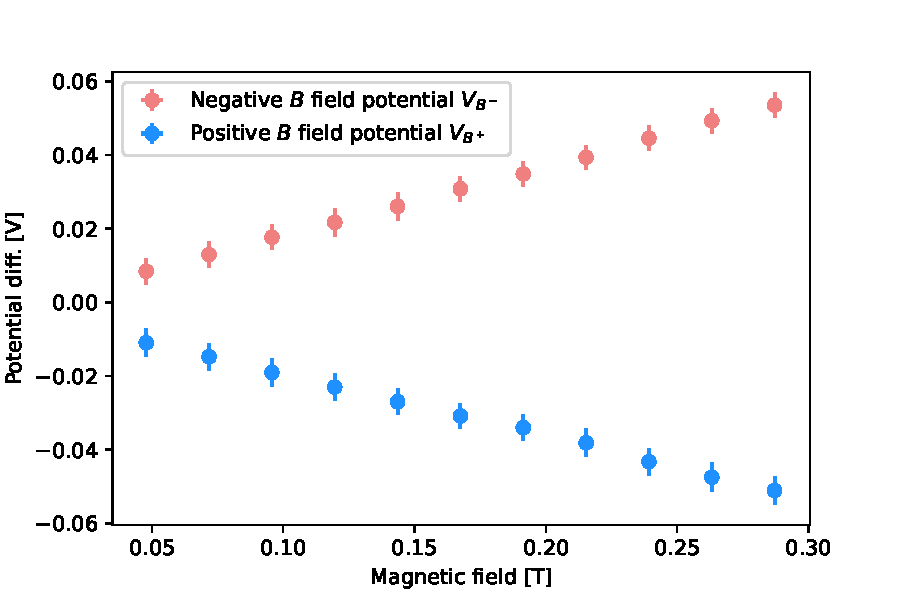
\includegraphics[width=\linewidth]{plt_BB_VH.pdf}\label{fig:plot_BB_VH}}
    \caption{\ref{sub@fig:magnet_picture} Schema dell'elettromagnete utilizzato per generare il campo magnetico $B$ (nell'esempio si vede la configurazione per ottenre $B^-$). \ref{sub@fig:plot_BB_VH} Plot dei valori di tensione misurati amplificati ai capi della sonda rispetto al valore del campo magnetico generato dall'elettromagnete. Si può osservare il comportamento atteso per cui applicando un campo magnetico positivo o negativo, la tensione risulta essere positiva o negativa, coerentemente con la teoria.}
\end{figure}

Abbiamo considerato fino ad ora i portatori di carica aventi la stessa carica dell'elettrone $e$, senza però compiere nessuna ipotesi sul segno dei portatori stessi. Questo dato può unicamente essere ricavato eseguendo correttamente delle considerazioni sull'orientamento nello spazio dei campi $\vec{B}$ e $\vec{J}$ e sull'orientamento di $E_H$ essendo misurato il potenziale $V_H$. Consideriamo sempre il sistema ortonormale della figura \ref{fig:sonda.rotated}, allora abbiamo che la corrente spinge i portatori di carica lungo la direzione positiva di $\hat{e}_1$. Il secondo fattore che entra in gioco è quindi il campo magnetico, ovvero il suo orientamento, nel determinare come sarà fatta la forza di Lorentz (\ref{eq:lorentz_F_m}). Questo orientamento possiamo ottenerlo conoscendo in quale verso scorre la corrente all'interno della bobina dell'elettromagnete. Osserviamo però che, nel caso in cui la corrente scorra in senso antiorario nelle bobine (viste dell'altro) allora il campo magnetico sarà diretto verso l'alto all'interno delle bobine e, per continuità, diretto verso il basso alll'interno del traferro. Siamo quindi nel caso per cui $B=B^-$, ovvero $\vec{B} = -B\hat{e}_2$. In questo caso allora la forza di Lorentz sarà quindi proporzionale a $-\hat{e}_3$. Ipotizzando che le nostre cariche siano negative, dovremmo osservare allora che aumentando il valore del campo magnetico il valore della tensione di Hall diventa mano a mano minore (dovremmo effettivamente osservare un valore della tensione negativo, che però per quanto detto in \ref{sec:vlong}). Viceversa se invece consideriamo la corrente che scorre nelle bobine diretta come $\vec{B}=B\hat{e}_2$ allora otterremmo che $\vec{F}_m \propto \hat{e}_3$, quindi osservando, sempre nell'ipotesi di cariche negative, una tensione lungo $\hat{e}_3$ positiva. Dai dati raccolti sperimentalmente osserviamo (figura \ref{fig:plot_BB_VH}) un comportamento coerente con quanto previsto teoricamente, quindi possiamo confermare che i portatori di carica presentano segno negativo, trattandosi quindi di elettroni. 

\section{Calcolo di $\mathbf\eta$ e conclusioni}\label{sec:computing_eta_and_conlusion}

\begin{figure}
    \centering
    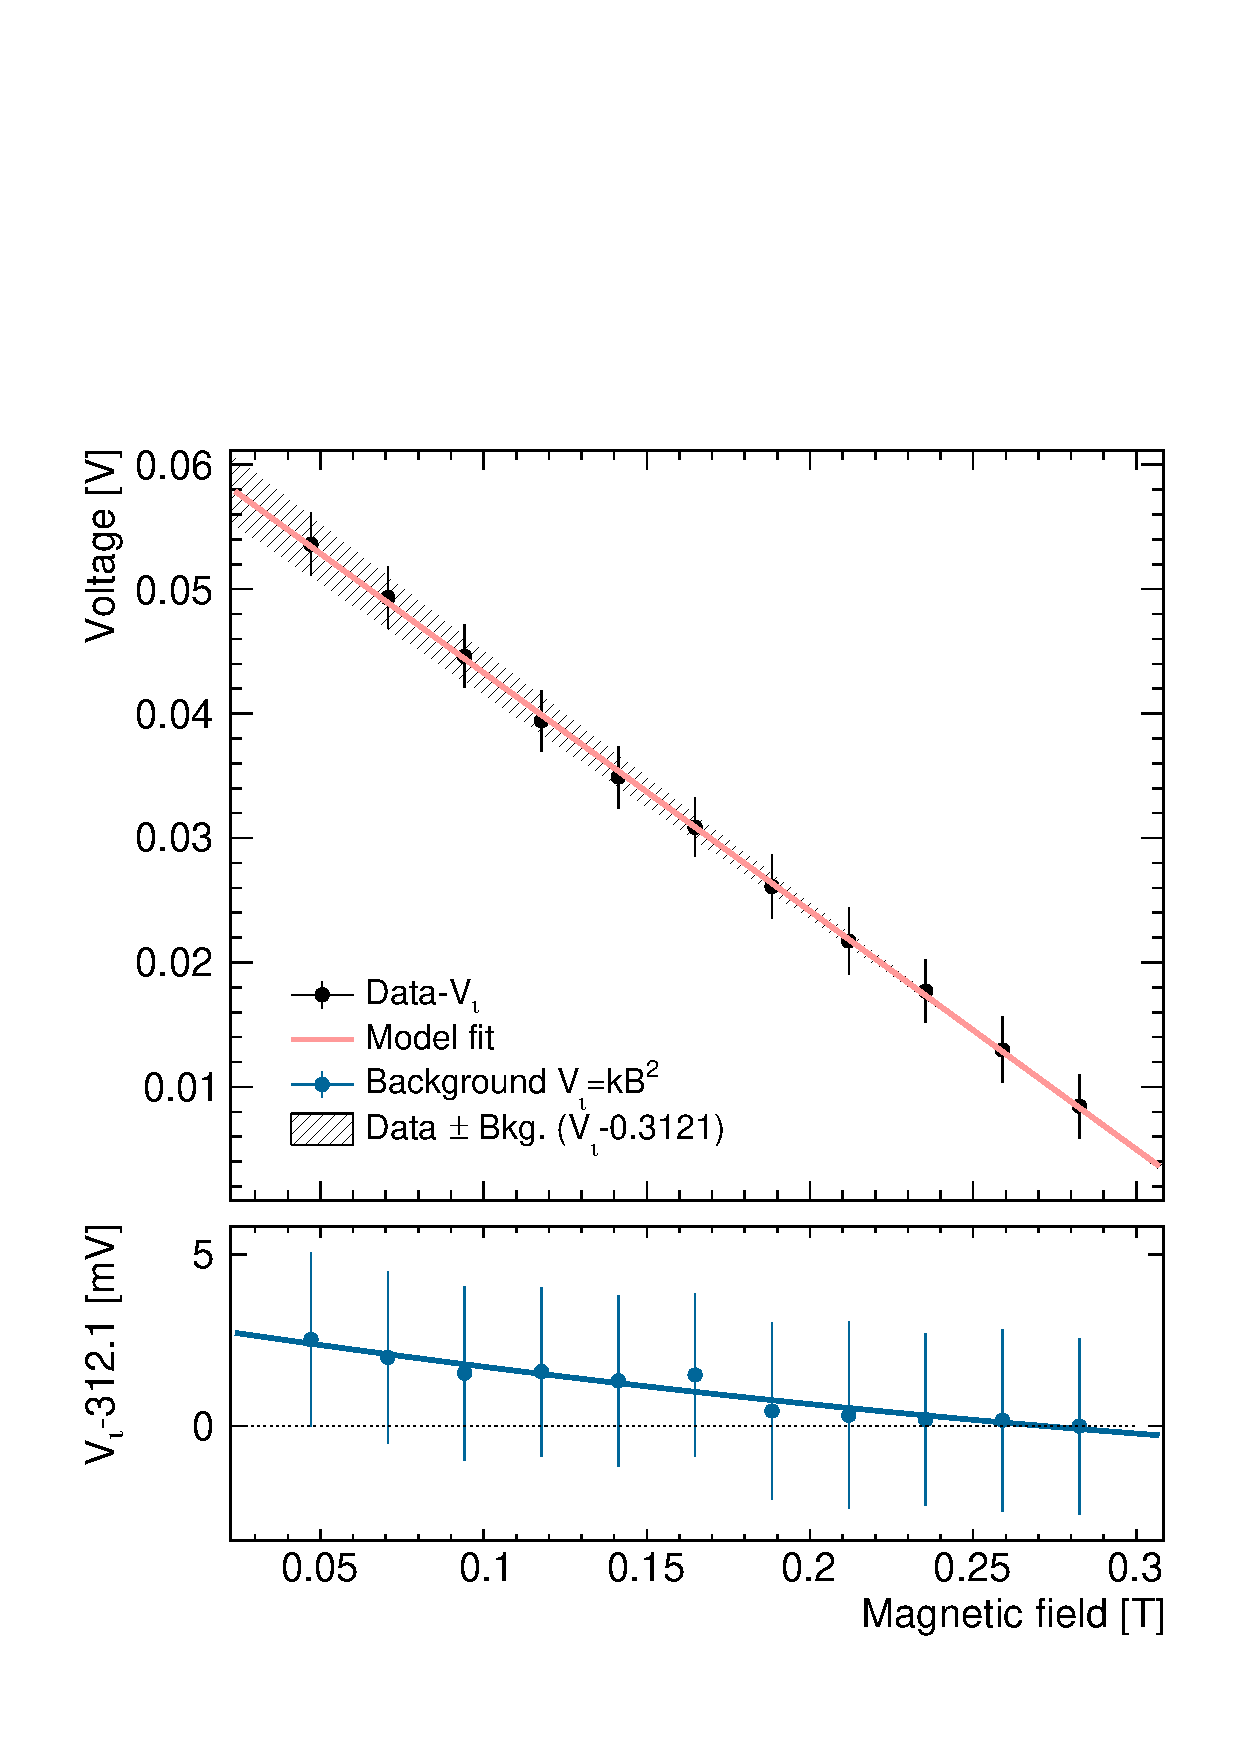
\includegraphics[width=\linewidth]{plot_vb.pdf}
    \caption{Dipendenza lineare della tensione di Hall (rappresentata con un guadagno di $G_\text{diff} = \num{2.07(24)e2}$) dal campo magnetico prodotto dall'elettromagnete. I valori di tensione sono ottenuti eliminando la componente quadratica, che viene isolata sotto (i dati per $V_\ell$ sono riscalati portando il valore più basso a zero). Possiamo infatti osservare un andamento quadratico della componente di background $V_\ell$ che permette quindi anche di stimare il parametro $k$.}\label{fig:plot_vb}
\end{figure}

Considerando una sonda di spessore $w=\SI{4.500(115)}{\micro\metre}$ sottoposta al campo magnetico generato dall'elettromagnete descritto sopra, alimentato con correnti da \SI{0.2}{\tesla} a \SI{1.2}{\tesla}, possiamo allora ottenere una misura della tensione $V_{G,H}$ lungo $\hat{e}_3$ sul rivelatore. Se eliminiamo la componente quadratica $kB^2$ dalla relazione (\ref{eq:full_fit}), allora dall'eq. (\ref{eq:2}), considerando $V_{G,H} = V_{G,H}(B)$, possiamo ricavare, da un modello lineare, il coefficiente di proporzionalità $C$ che contiene al suo interno tutte le informazioni legate alle caratteristiche della sonda, della corrente $i$ e della densità di portatori $\eta$, oltre che dal guadagno dell'amplificatore. In figura \ref{fig:plot_vb} i dati sono rappresentati già in seguito all'eliminazione della componente quadratica $V_\ell$, che viene invece isolata nel grafico sottostante per mettere in evidenza l'andamento quadratico. 

\begin{table*}
    \caption{Parametri utilizzati nel fit del modello (\ref{eq:model_fit}) per ricavare il valore di $\eta$.}\label{tab:model_parameters}
    \begin{ruledtabular}
        \begin{tabular}{lll}
            Quantità & Valore & \\\colrule
            Carica elettrone & \SI{1.602176634e-19}{\coulomb} & Fonte: \cite{Newell_2018}\\
            Spessore della sonda & \SI{4.500(115)}{\micro\metre} & \\
            Corrente & \SI{8.619(150)}{\milli\ampere} & Calcolata da $G_g = \SI{1.7242(300)}{\milli\ampere \per\volt}$ (Appendice \ref{sec:appendix_current_gen}).\\
            Guadagno differenziale & \num{2.06551(0.244501)e2} & Appendice \ref{sec:appendix_strum_opamp}.\\
        \end{tabular}
    \end{ruledtabular}
\end{table*}

Adattando il modello lineare (\ref{eq:model_fit}) possiamo allora ricavare il coefficiente $C$, e quindi, noti i parametri di costruzione della sonda e del setup sperimentale (raccolti in tabella \ref{tab:model_parameters}) possiamo calcolare il valore \begin{equation}
    \eta = \SI{1.310(175)e+25}{\per\cubic\metre}.\label{eq:result}
\end{equation} Osserviamo però che dalla figura \ref{fig:plot_vb} la tensione di Hall sembra essere decrescente all'aumentare di $B$ nel traferro. Questo è solamente legato a come si sono ricavati i dati privati della componente $kB^2$, infatti, invertendo i segni nella relazione (\ref{eq:model_fit}) otterremmo che il potenziale risulta crescere (la differenza di potenziale è effettivamente presa a meno di una costante, che quindi può far cambiare il segno dei dati ottenuti). 

Passando invece a considerare il termine $kB^2$ possiamo innanzitutto osservare che questo contributo è decisamente rilevante, tanto da fare si che sia con $B^+$ sia con $B^-$ i valori misurati di tensione fossero positivi per tutti i valori del campo magnetico. Possiamo quindi ipotizzare che il difetto legato alla forma della sonda non sia trascurabile, o che comunque una variazione molto piccola (solo qualche decina di \si[]{\micro\metre}) porti ad osservare una tensione molto maggiore dell'effetto di Hall (un valore medio di circa \SI{320}{\milli\volt} rispetto ad una variazione totale legata al fenomeno di Hall di $\simeq\SI{50}{\milli\volt}$). Modellando una curva parametrica di secondo ordine sui dati ottenuti isolando il termine $kB^2$ otteniamo un valore del coefficiente \begin{equation}
    k=\SI{11.88(3.82)}{\volt\per\tesla\squared}.
\end{equation}

Ritornando ad analizzare infine il valore trovato di $\eta$ in (\ref{eq:result}) allora possiamo sicuramente dire che tale valore risulta essere piuttosto sensato, otteniamo infatti un valore che si trova intorno agli ordini di grandezza di altre densità di portatori di altri elementi come già detto in \footnotemark[10]. Allo stesso tempo però confrontando il valore ottenuto da altri risultati scientifici \cite{Hasegawa:2006tu,Michenaud:1972wx,Edelman:1977wy} con $\eta$ calcolato in (\ref{eq:result}), osserviamo che, seppur solo di solo un ordine di grandezza, non risultano essere compatibili.

%|||||||||||||||||||||||||||||||||||||||||||||||||||||||||||||||||||||||||||||||||||

%\onecolumngrid
\appendix
\renewcommand{\thefigure}{\thesection\arabic{figure}}

\section{Caratterizzazione del generatore di corrente}\label{sec:appendix_current_gen}

In figura \ref{fig:circuito_gen_i} è riportato lo schema circuitale del generatore di corrente. Tale circuito è tale per cui data una differenza di potenziale fornita al circuito come $V^{-}-V^{+}$ si ha in uscita una corrente $i_\text{out}=\frac{R_2}{R_1}\cdot \frac{V^--V^+}{R_5}$. Siccome abbiamo previsto che la tensione che forniamo al circuito è pari a \SI{5}{\volt} e vogliamo che la corrente cha va alla sonda non superi \SI{10}{\milli\ampere} allora il fattore $G_g=\frac{R_2}{R_1}\cdot\frac{1}{R_5}$ dovrà essere minore di \SI{2}{\milli\ampere\per\volt}. Scegliamo quindi $R_{1}=R_{2}=\SI{1}{\kilo\ohm}$ e $R_{5}=\SI{500}{\ohm}$. Per verificare se effettivamente il fattore $G_g$ sia pari a $1/500$ possiamo raccogliere una serie di coppie valori di $i_\text{out}$ e $V^{-}-V^{+}$ e realizzare un fit (figura \ref{fig:gen_i_model}) secondo la funzione $i_\text{out}=G_g\cdot \qty(V^--V^+) + i_0$ dove scegliamo come parametri di fit $G_{g}$ e $i_0$. Otteniamo che \begin{align*}
    G_g &=\SI{1.7242(300)}{\milli\ampere \per\volt}\\
    i_0 &= \SI{0.0673(889)}{\ampere}.
\end{align*} Il valore teorico di $G_g$ è \SI{1.783(124)}{\milli\ampere\per\volt} per cui troviamo che è compatibile con il valore ricavato dal fit e troviamo anche che il valore di $i_0$ è compatibile con zero, per cui possiamo dire che non c'è un offset sulla corrente che mandiamo alla sonda.
Un ulteriore test fatto è stato quello di mantenere costante il valore di $V^--V^+$ e verificare che, cambiando il carico in uscita dal generatore, la corrente rimane sempre la stessa.

\begin{figure}
    \centering
    \subfloat[][]{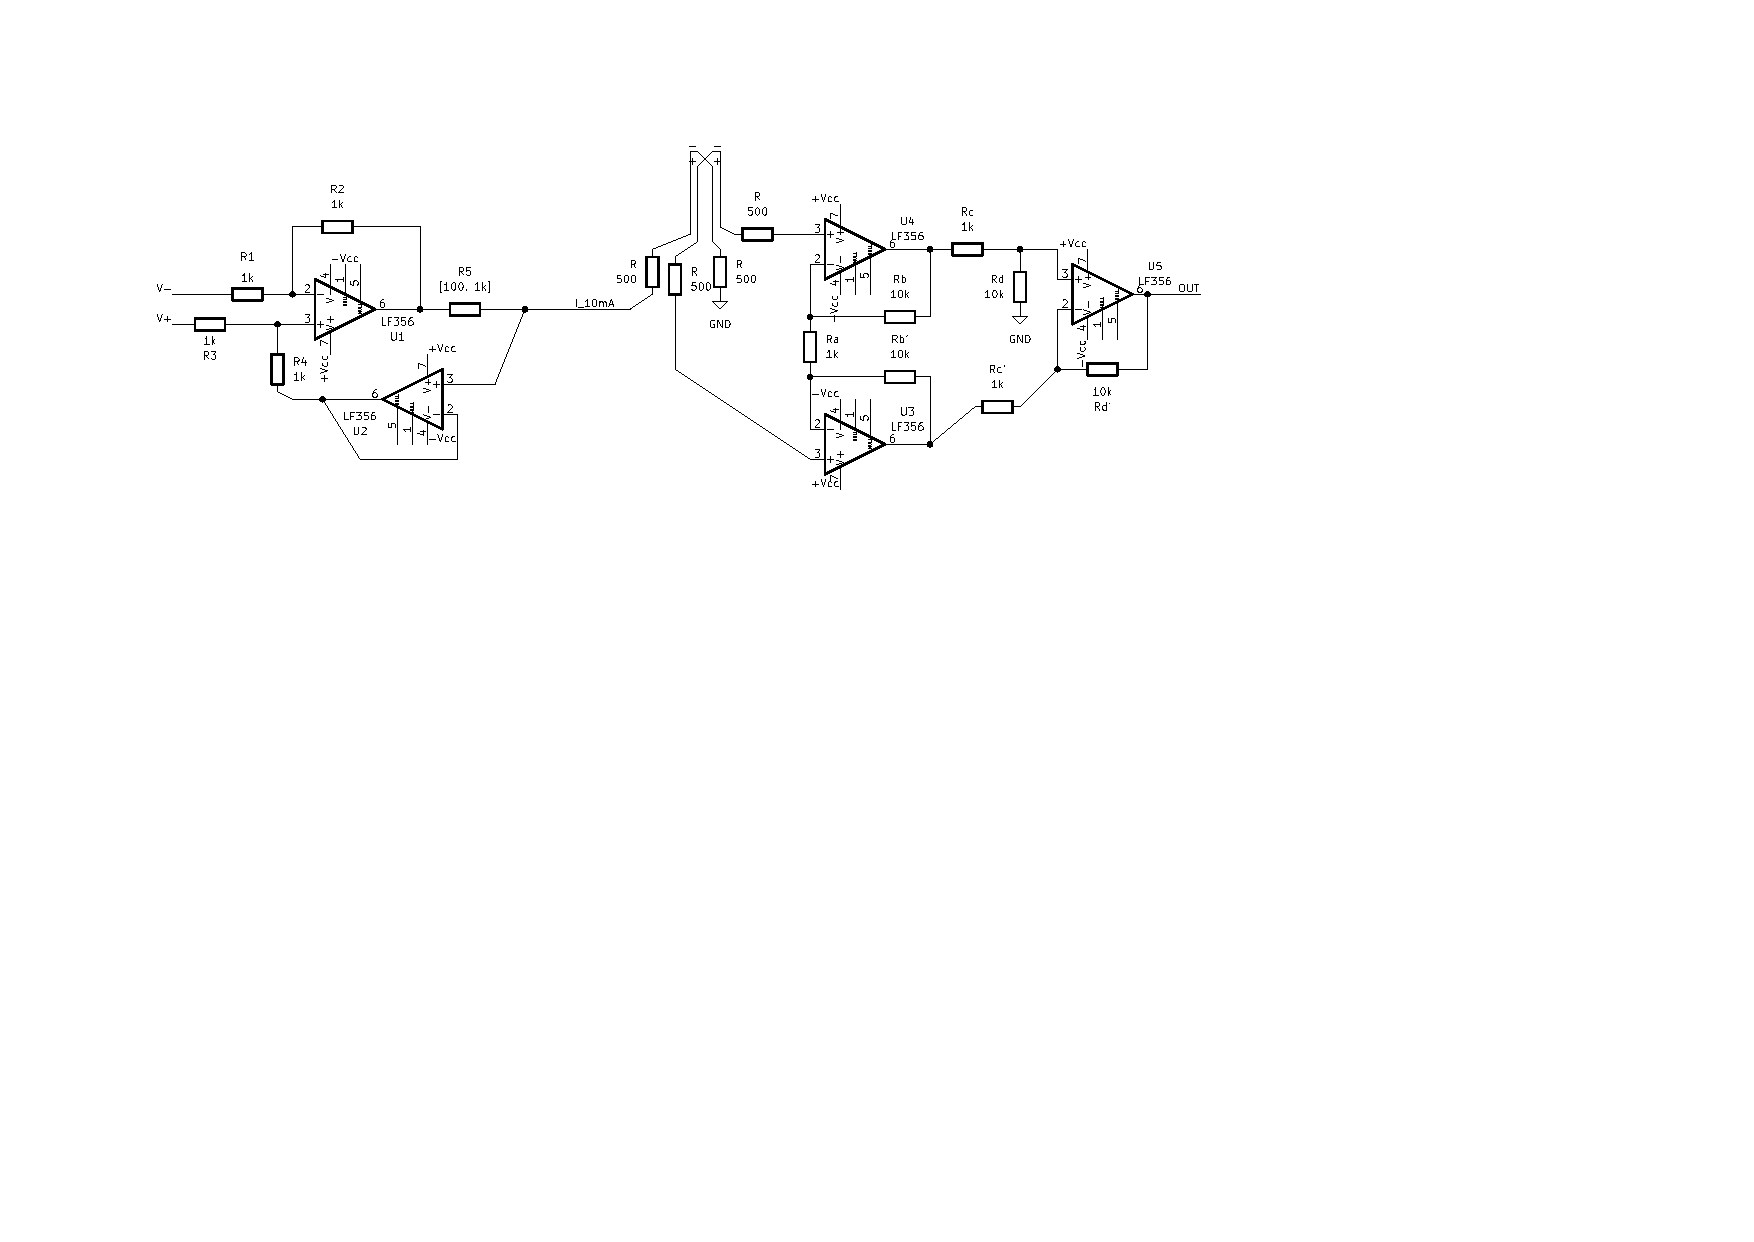
\includegraphics[width=0.85\linewidth,trim={1.8cm 13cm 20.35cm 2.5cm},clip]{SCHEMA_full1.pdf}\label{fig:circuito_gen_i}}\\
    \subfloat[][]{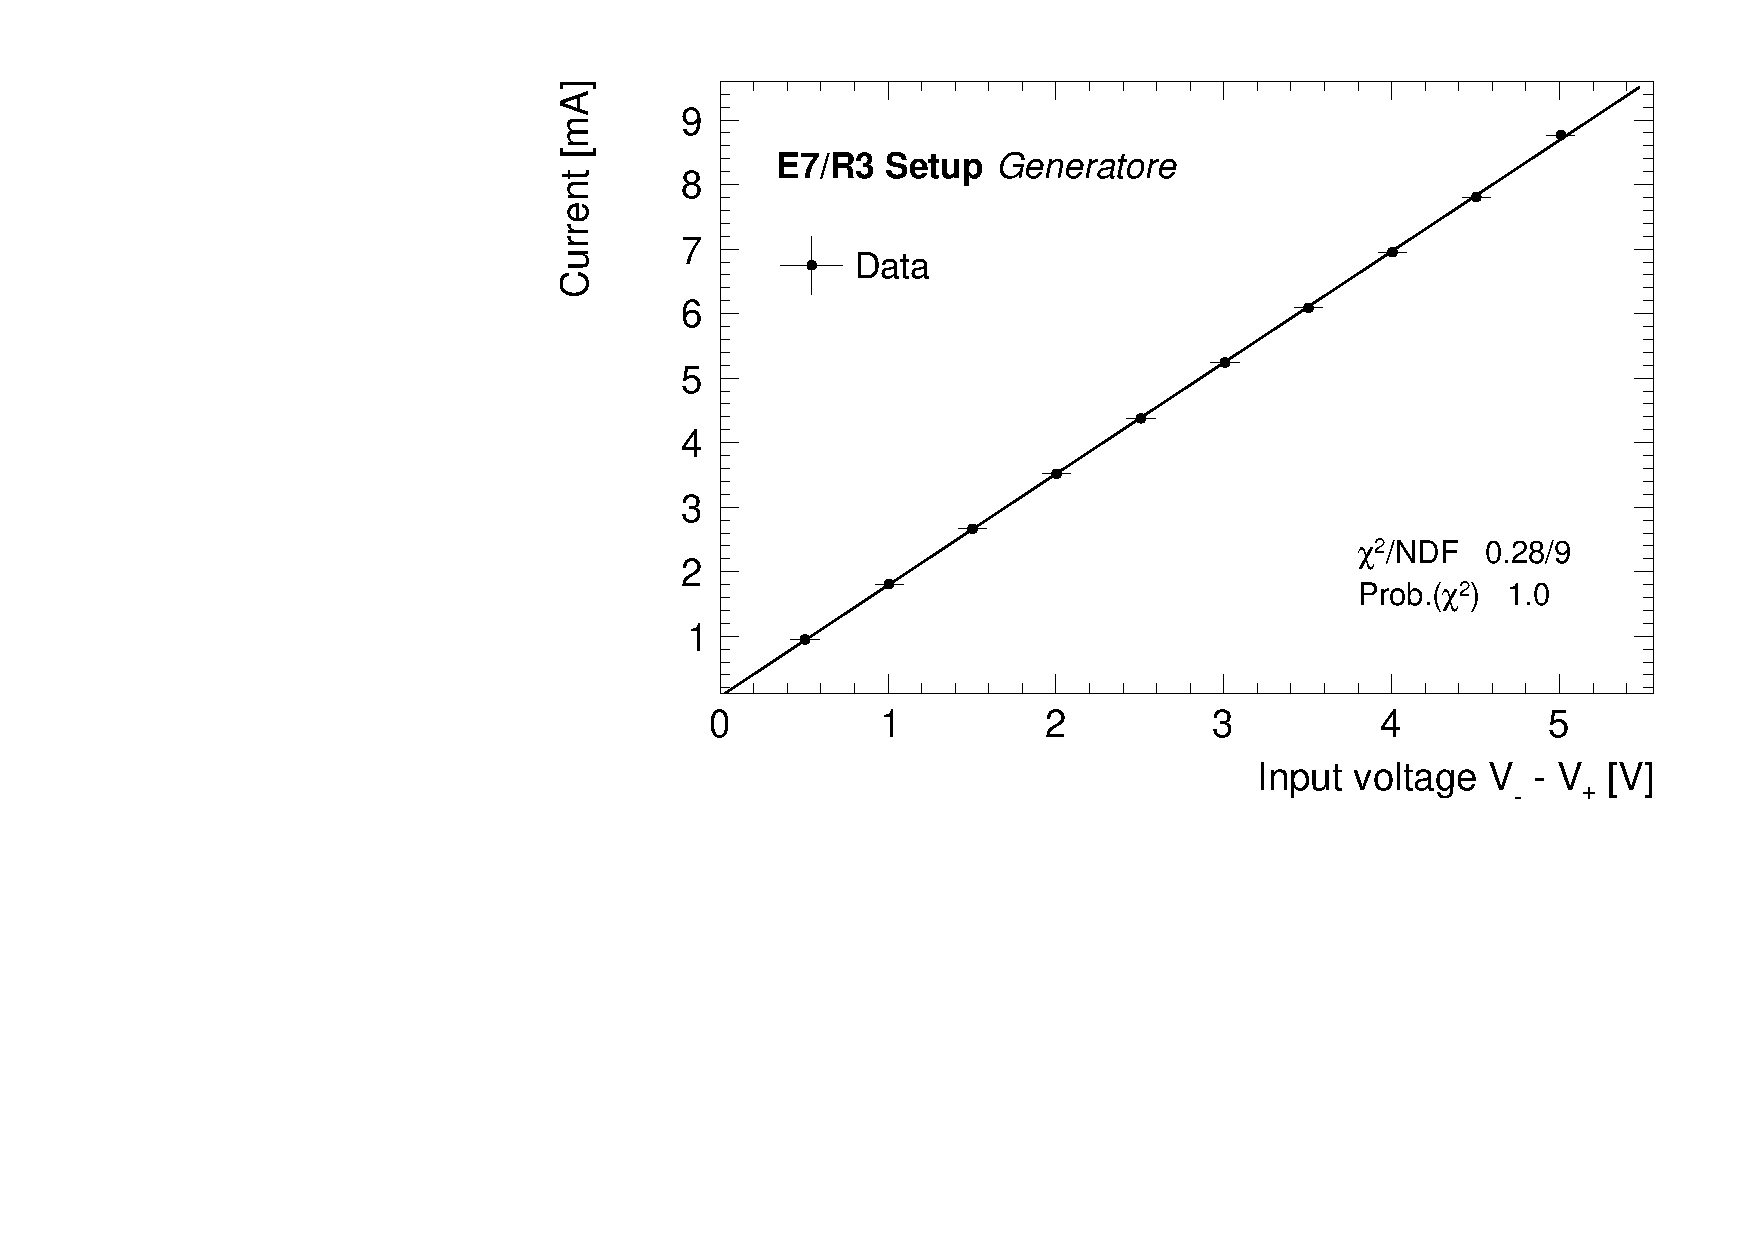
\includegraphics[width=\linewidth]{GEN.0.10mA.pdf}\label{fig:gen_i_model}}
    \caption{
        \ref{sub@fig:circuito_gen_i} Schema del circuito del generatore di corrente. L'uscita dalla resistenza $R_5$ porta la corrente di circa \SI{10}{\milli\ampere} alla sonda.
        \ref{sub@fig:gen_i_model} Caratterizzazione del generatore di corrente. 
    }
\end{figure}

%|||||||||||||||||||||||||||||||||||||||||||||||||||||||||||||||||||||||||||||||||||

\section{Caratterizzazione dell'amplificatore operazionale per strumentazione}\label{sec:appendix_strum_opamp}

In figura \ref{fig:circuit_amp} è riportato lo schema circuitale dell'amplificatore per strumentazione che  è caratterizzato da una funzione di trasferimento \begin{equation}
    V_\text{out} = G_\text{diff}\cdot \qty(V_\text{non-inv}-V_\text{inv}) +  G_\text{CM}\cdot V_\text{CM} + V_\text{offset} 
\end{equation}
La parte predominante di $V_\text{out}$ è data da $G_\text{diff}\qty(V_\text{non-inv}-V_\text{inv})$ dove $G_\text{diff}$, se $R_b=R_b'$, $R_c=R_c'$ e $R_d=R_d'$, è pari a $\frac{R_{d}}{R_{c}}\cdot \qty(1+2\cdot \frac{R_{b}}{R_{a}})$. Siccome vogliamo amplificare il segnale in uscita dalla sonda di circa 200 volte scegliamo resitenze da \SI{1}{\kilo\ohm} per $R_a$, $R_c$ e da \SI{10}{\kilo\ohm} per $R_b$ e $R_d$. Per caratterizzare l'amplificatore è necessario trovare quali sono gli effettivi valori di $V_\text{offset}$, $G_\text{CM}$ e $G_\text{diff}$. 
Per trovare $V_\text{offset}$ fissiamo $V_\text{non-inv}=V_\text{inv}=0$ e osserviamo che il valore misurato è nell'ordine dei \si{\milli\volt}. Per far diminuire ancora di più questo valore possiamo utilizzare un trimmer (una resistenza variabile che corregge le differenze di impedenza presenti tra i due amplificatori operazionali del primo stadio) presente sul circuito stampato in modo che $V_\text{offset}$ sia più prossimo possibile a zero.
Per trovare invece $G_\text{CM}$ impostiamo $V_\text{non-inv}=V_\text{inv}\neq 0$ e raccogliamo una serie di coppie di valori $(V_\text{non-inv/inv},V_\text{out})$ realizzando un fit secondo la funzione $V_\text{out}=G_\text{CM}\cdot V+V_0$, dove $G_\text{CM}$ e $V_0$ sono i parametri. Dal fit (figura \ref{fig:GCM_plot}) otteniamo \begin{align*}
    G_\text{CM} &= \num{-1.12226(0.204461)e-2}\\
    V_0 &= \SI{4.52655(4.53222)e-3}{\volt}
\end{align*}

Notiamo che come ci aspettavamo $V_0$ è compatibile con zero.
Per trovare $G_\text{diff}$  raccogliamo alcune coppie di valori $(V_\text{non-inv}-V_\text{inv},V_\text{out})$ e, facendo un fit (figura \ref{fig:Gdiff_plot}) secondo la funzione $V_\text{out}=G_\text{diff}\cdot (V_\text{non-inv}-V_\text{inv})+V_0$, otteniamo \begin{align*}
    G_\text{diff} &= \num{2.06551(0.244501)e2}\\
    V_0 &= \SI{-1.49456(0.866213)}{\volt}
\end{align*}

Il valore teorico di $G_\text{diff}$ ottenuto dai valori di progetto e dalle misure delle resistenze risulta essere \num{2.09(.10)e2}, che osserviamo essere perfettamente compatibile con il valore che abbiamo ottenuto. 

\begin{figure}
    \centering
    \subfloat[][]{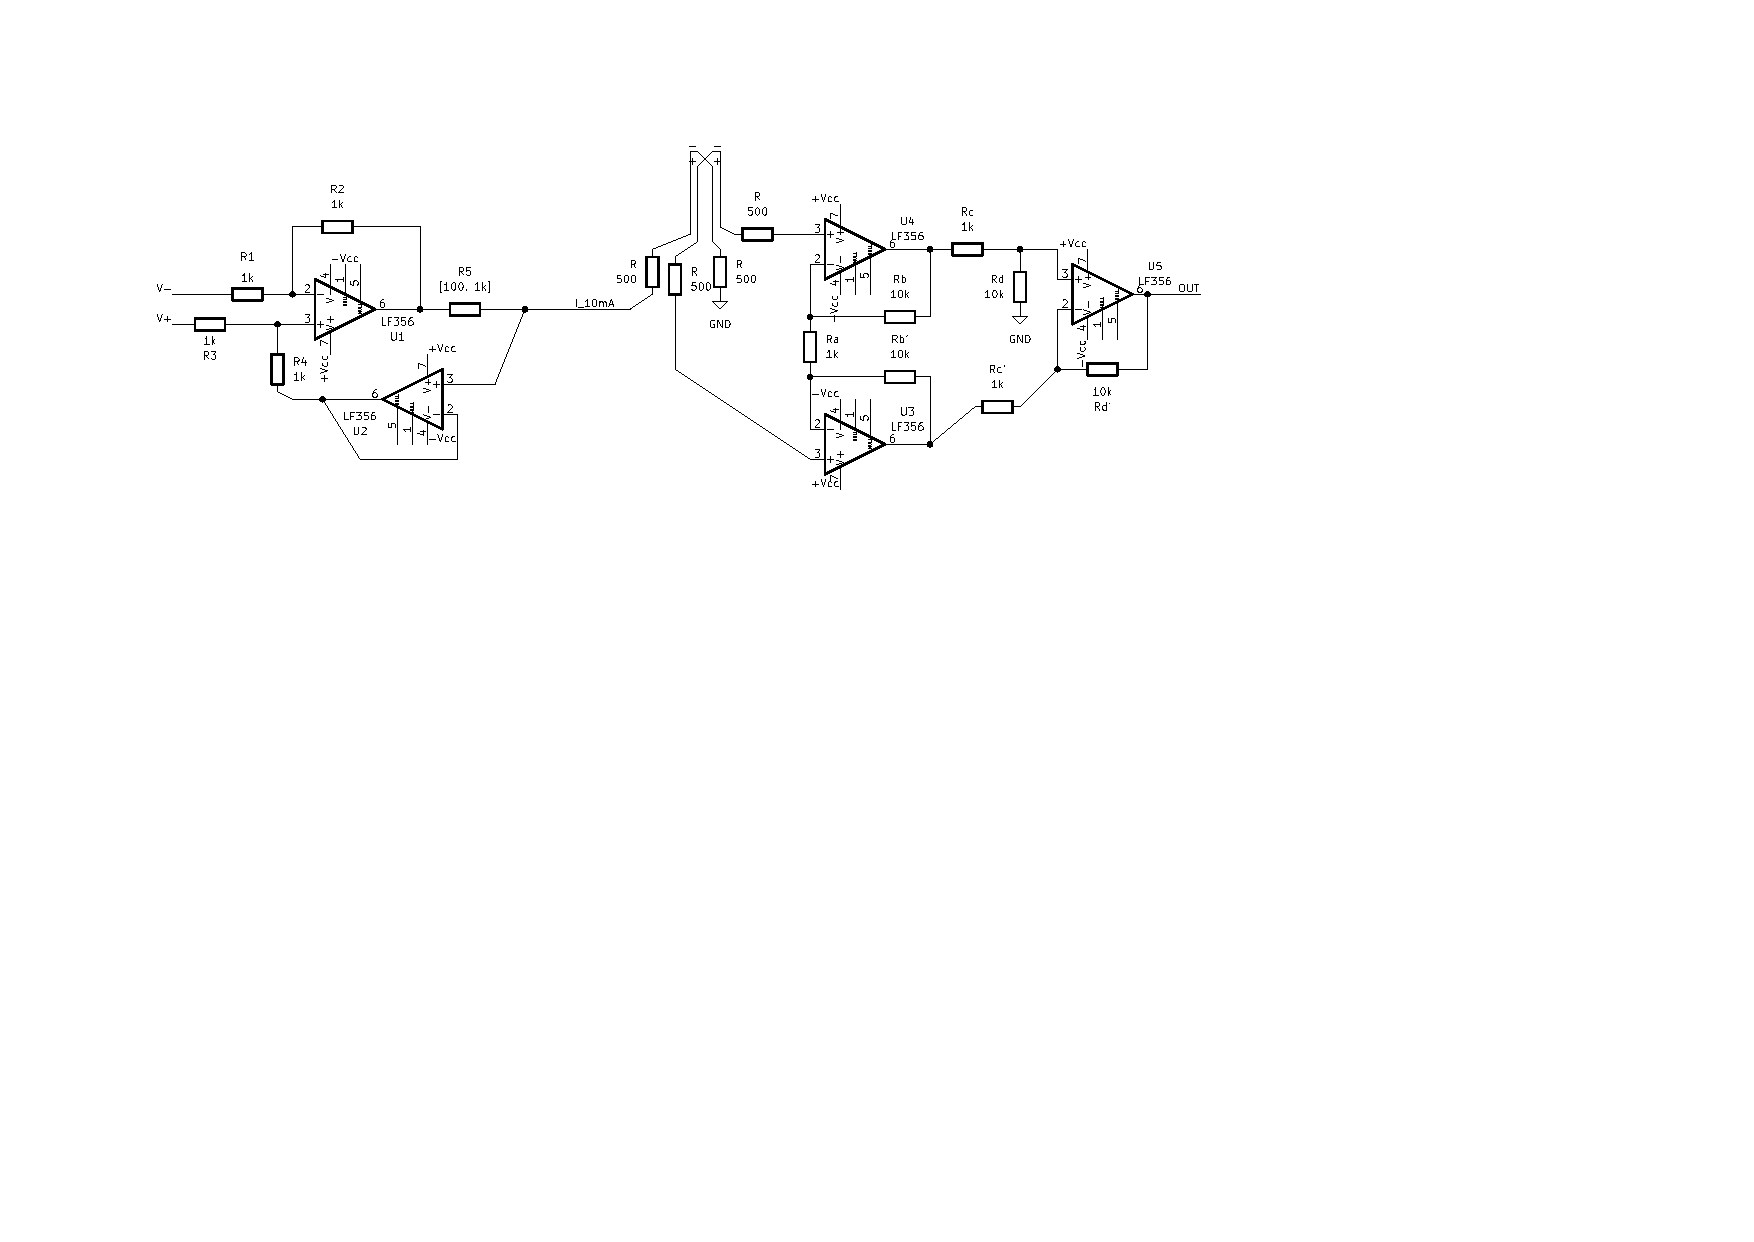
\includegraphics[width=0.85\linewidth,trim={18.65cm 12.75cm 3.5cm 2.25cm},clip]{SCHEMA_full1.pdf}\label{fig:circuit_amp}}\\
    \subfloat{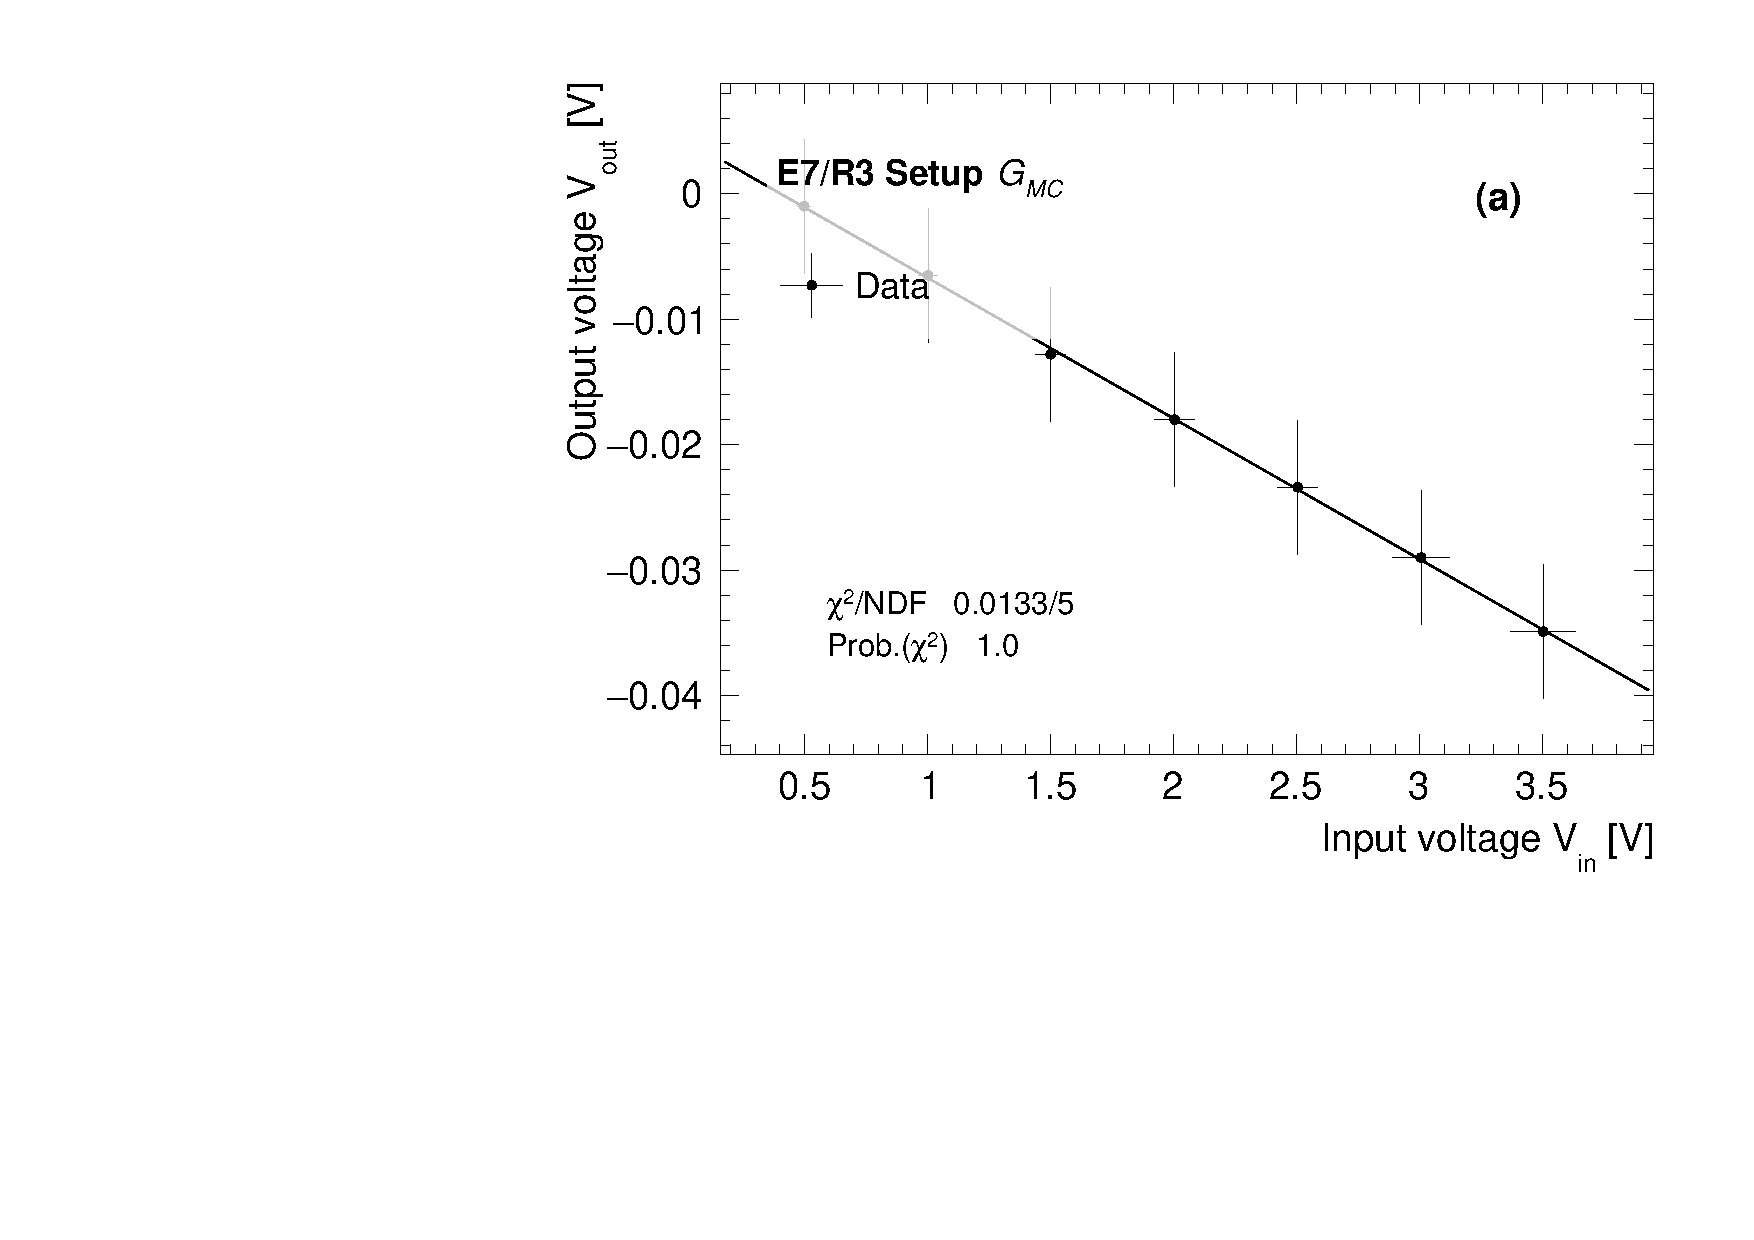
\includegraphics[width=\linewidth]{G_CM.pdf}\label{fig:GCM_plot}}\\
    \subfloat{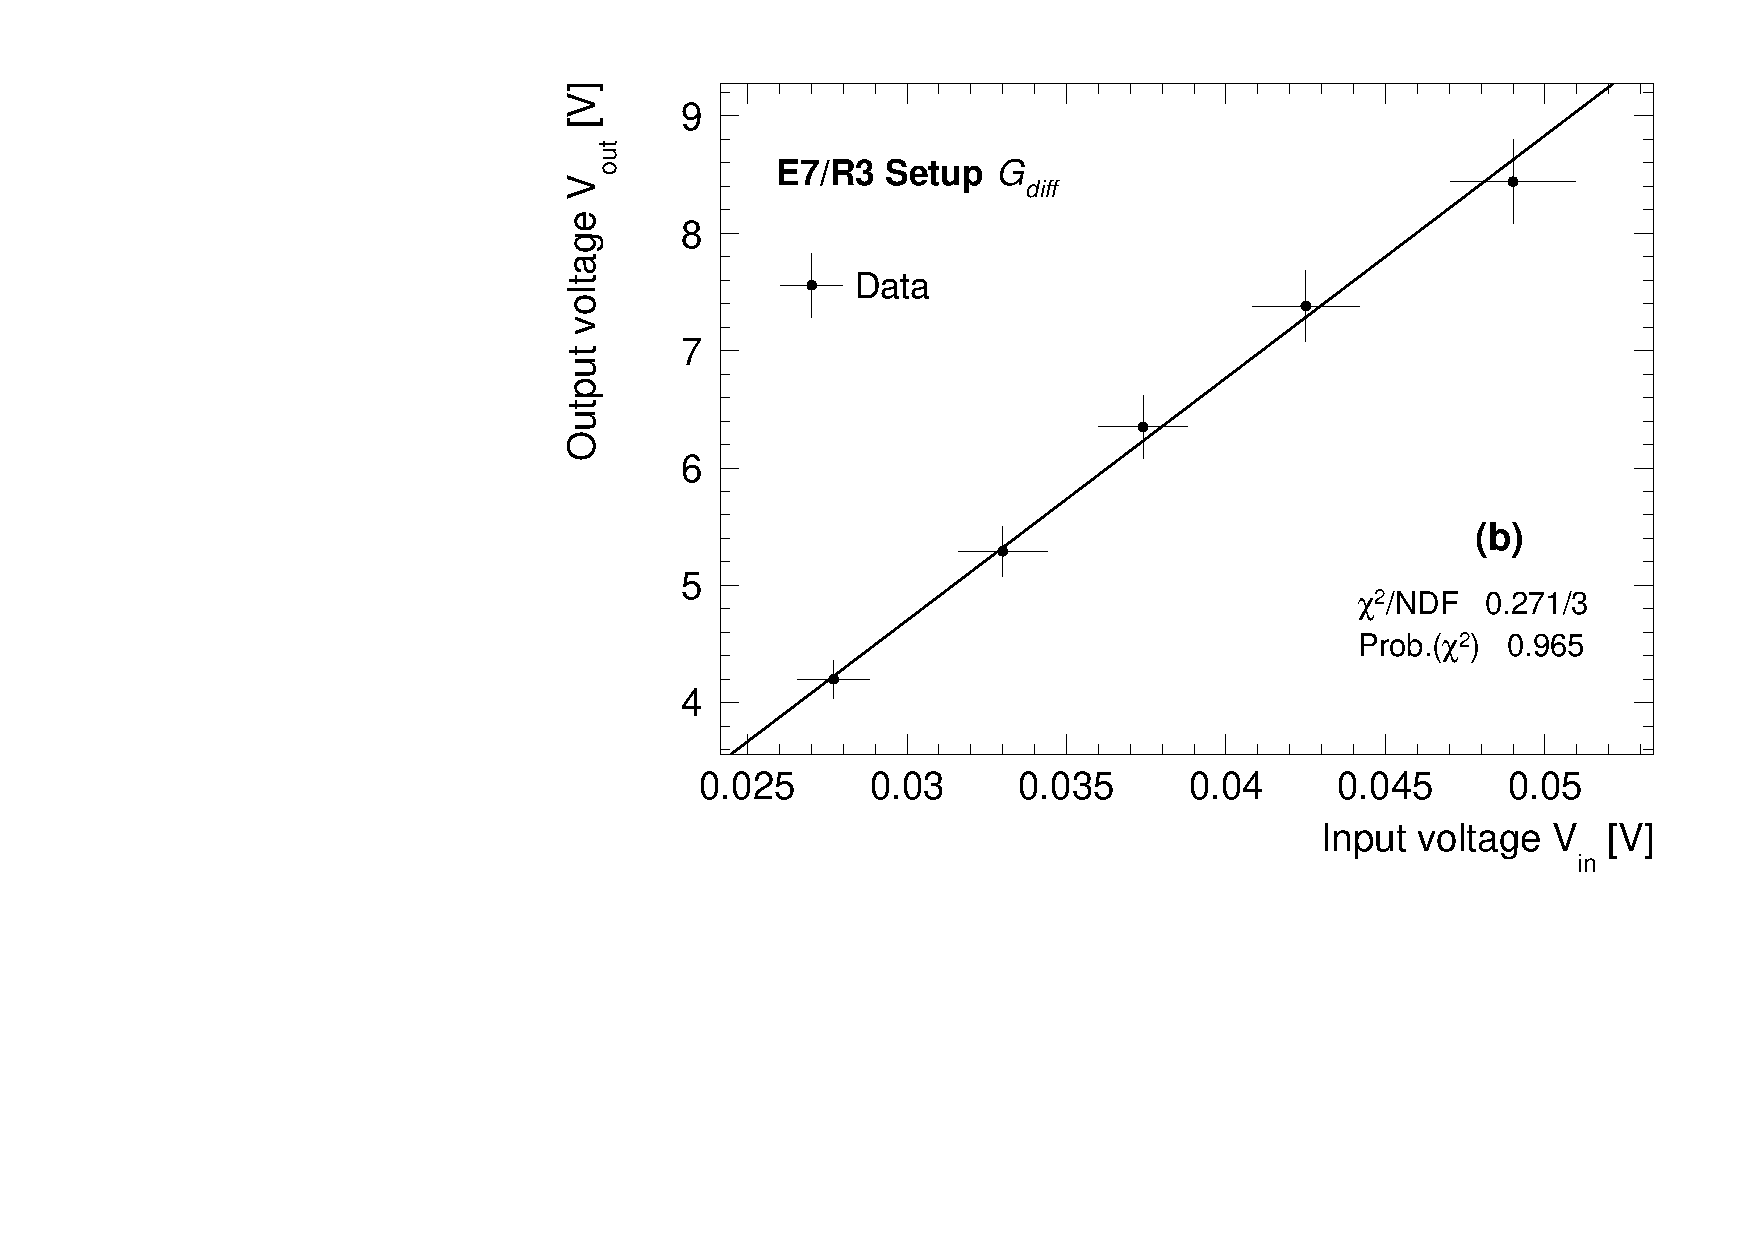
\includegraphics[width=\linewidth]{G_diff.pdf}\label{fig:Gdiff_plot}}

    \caption{
        \ref{sub@fig:circuit_amp} Schema circuitale dell'amplificatore operazionale per strumentazione.
        Analisi del guadagno di modo comune \ref{sub@fig:GCM_plot} e del guadagno differenziale \ref{sub@fig:Gdiff_plot} dell'amplificatore operazionale per strumentazione. 
    }
\end{figure}

%|||||||||||||||||||||||||||||||||||||||||||||||||||||||||||||||||||||||||||||||||||
% \iffalse
\section{Logica di controllo del setup sperimentale}\label{sec:control_logic}

Riportiamo  in nell'algoritmo \ref{alg:logic} la logica di controllo del micro-controllore Arduino MEGA 2560 che permette di automatizzare la presa dati.

\begin{algorithm}
    \DontPrintSemicolon
    \SetKwArray{AVoh}{$V_\text{out}$}
    \SetKwArray{AVol}{$V_\text{out}^{i=0}$}
    \SetKwArray{AVgh}{$V_\text{gen}$}
    \SetKwArray{AVgl}{$V_\text{gen}^{i=0}$}
    \SetKw{SetMode}{set}
    \SetKw{CreateMode}{create}
    \SetKw{Waitfor}{wait for}
    \SetKw{Inc}{increment}
    \SetKw{Dec}{decrement}
    \SetKwBlock{BRead}{read}{}
    \KwData{analog pins Arduino MEGA 2650}
    \KwResult{serial write $\to$ ROOT TFile with TTree structure}
    \CreateMode TTree $\gets$ "dataBpos"\;
    \SetMode $i_B=\SI{1.3}{\ampere}$\;
    \For(){$M=12$ cycles \emph{over} $m$}{
        \For(){$N=100$ cycles \emph{over} $n$}{
            \SetMode $i<\SI{10}{\milli\ampere}$ using digital \SI{5}{\volt} output\;
            \BRead{
                \AVoh{n} $\gets$ op-amp out\;
                \AVgh{n} $\gets$ digital \SI{5}{\volt} out\;
            }
            \SetMode $i=\SI{0}{\volt}$ (turn off digital out)\;
            \BRead{
                \AVol{n} $\gets$ op-amp out\;
                \AVgl{n} $\gets$ digital \SI{5}{\volt} out\;
            }
            \KwOut{write data $\to$ TBranches}
            \Inc $i:=i+\SI{0.1}{\volt}$
        }
    }
    \Waitfor{$\Delta t = \SI{45}{\second}$: invert $B$ field polarity}\;
    \CreateMode TTree $\gets$ "dataBneg"\;
    \For(){$M=12$ cycles \emph{over} $m$}{
        \For(){$N=100$ cycles \emph{over} $n$}{
            \SetMode $i<\SI{10}{\milli\ampere}$ using digital \SI{5}{\volt} output\;
            \BRead{
                \AVoh{n} $\gets$ op-amp out\;
                \AVgh{n} $\gets$ digital \SI{5}{\volt} out\;
            }
            \SetMode $i=\SI{0}{\volt}$ (turn off digital out)\;
            \BRead{
                \AVol{n} $\gets$ op-amp out\;
                \AVgl{n} $\gets$ digital \SI{5}{\volt} out\;
            }
            \KwOut{write data $\to$ TBranches}
            \Dec $i:=i-\SI{0.1}{\volt}$
        }
    }
    \KwResult{ROOT TFile $\gets$ ("dataBpos", "dataBneg")}
    \vspace{0.5cm}
    \caption[]{Logica di controllo del setup sperimentale.}\label{alg:logic}
\end{algorithm}
% \fi

%\bibliographystyle{plain}
\bibliography{references/IOP.shortcomm.CODATA2017, references/10.2307_2369245, references/results.bib}

\begin{methods}{D\lowercase{ati completi e codice sorgente}}
    Tutti i dati completi a supporto dei grafici, e il relativo codice, sono visualizzabili su \url{https://github.com/mattiasotgia/Lab2}. L'analisi dati viene eseguita attraverso diversi notebook (\url{https://jupyter.org/}) scritti in C++/python basandosi su framework pubblici: ROOT, per la realizzazione dei grafici e il fit dei modelli (\url{https://root.cern/}), matplotlib, numpy e altri framework pubblici per l'analisi dei dati e la loro visualizzazione (\url{https://matplotlib.org/}, \url{https://numpy.org/}). I dati sono raccolti su file ROOT organizzati in dataset tabulari. Sono utilizzate anche le librerie uproot e Awkward Array (\url{https://uproot.readthedocs.io/}, \url{https://awkward-array.org/}).
\end{methods}

\end{document}
    
